\documentclass[12pt,a4paper]{article}
\usepackage{graphicx}
\usepackage{geometry}
\usepackage{caption}
\usepackage{booktabs}
\usepackage{longtable}
\usepackage{xcolor}
\usepackage{hyperref}
\usepackage{amsmath}
\geometry{margin=1in}

\title{Supplementary Materials:\\Evidence-Based Interpretation Framework for Lenacapavir Resistance}
\author{}
\date{}

\begin{document}
\maketitle

\noindent\textbf{Contents:}
\begin{enumerate}
  \item Figure S1. Data Harmonization Workflow
  \item Figure S2. Observation Counts by Mutation and Context
  \item Figure S3. Bootstrap Ranking Stability
  \item Figure S4. Expanded Structural Classification by Mechanism
  \item Figure S5. Full Interaction Network
  \item Figure S6. Validation Roadmap
  \item Figure S7. Sensitivity Analysis of Mutation Ranking Stability
  \item Table S2. Genetic Barrier Scores
  \item Table S3. Study Characteristics
  \item Table S4. Per-Mutation Summary Statistics
  \item Table S5. Complete Harmonized Phenotype Dataset
  \item Table S6. Multi-Mutant Phenotypic Observations
\end{enumerate}

\newpage

% ============================================================
% FIGURE S1
% ============================================================
\begin{figure}[!ht]
\centering
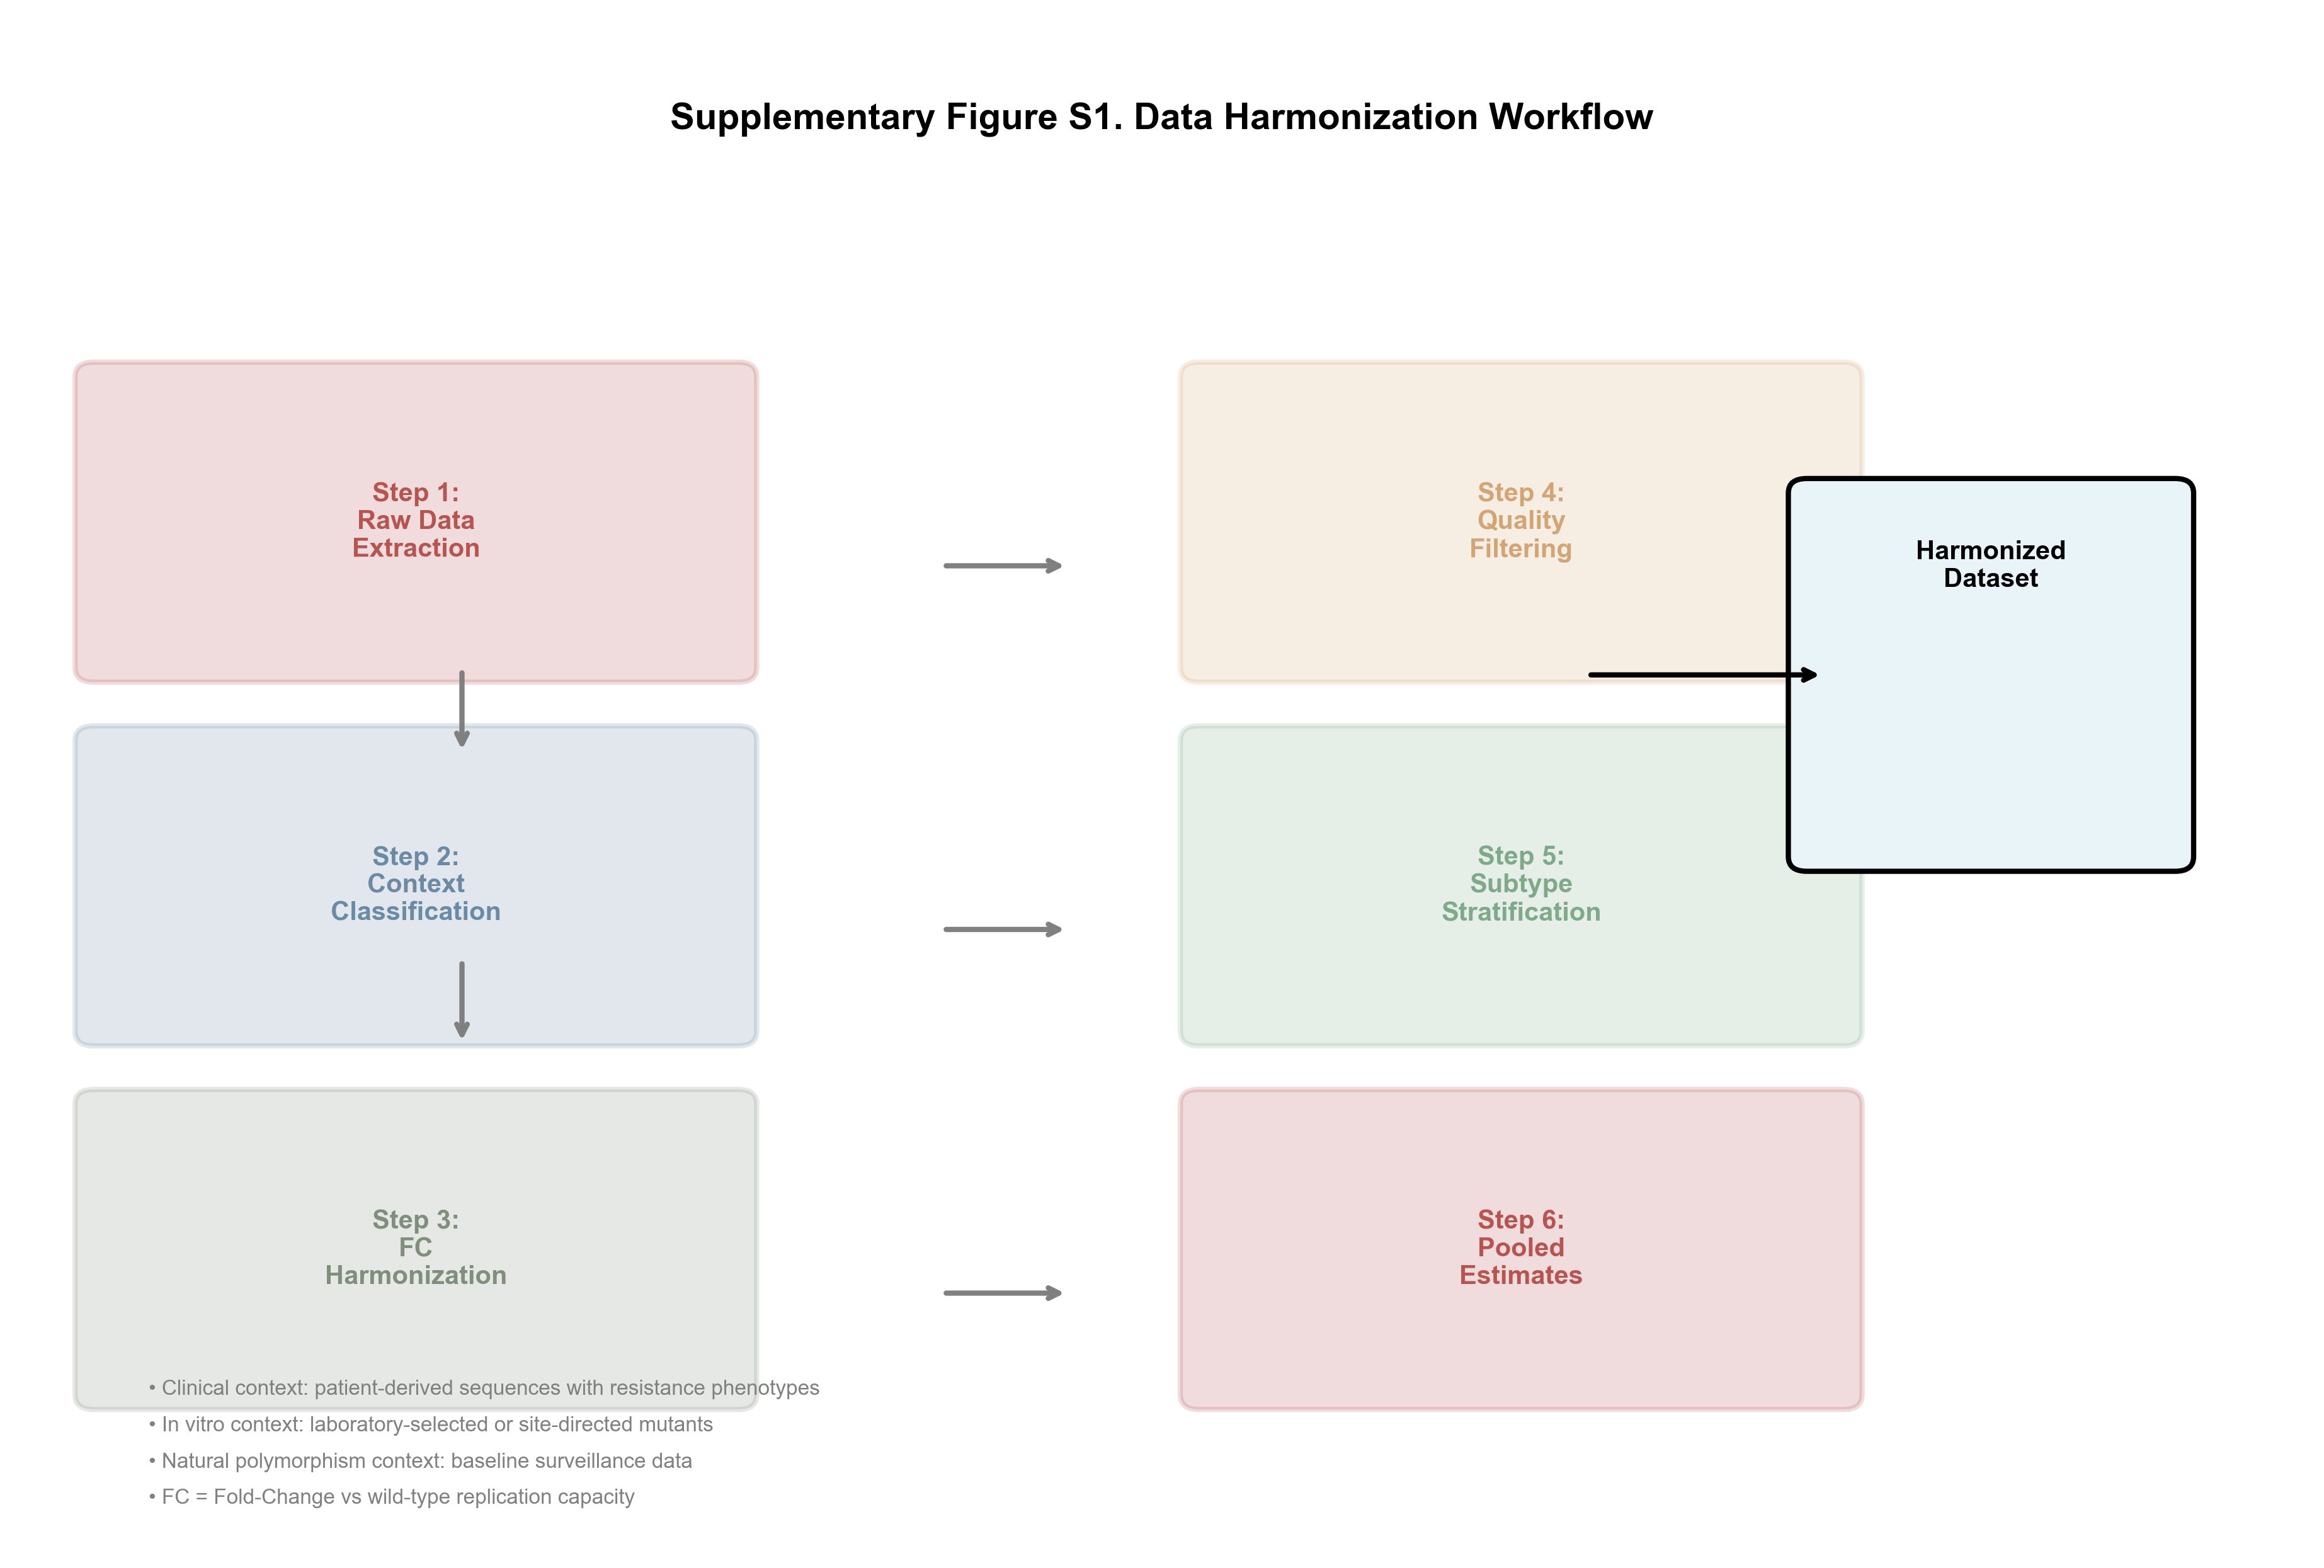
\includegraphics[width=0.95\textwidth]{supplementary/figures/figure_s1_harmonization.pdf}
\caption{\textbf{Data Harmonization Workflow.}
Schematic diagram showing the six-step pipeline for data extraction, context classification, fold-change harmonization, quality filtering, subtype stratification, and pooled estimate generation. Clinical context (patient-derived sequences with resistance phenotypes), in vitro context (laboratory-selected or site-directed mutants), and natural polymorphism context (baseline surveillance data) are distinguished. FC = EC$_{50}$ fold-change vs wild-type susceptibility (higher values indicate greater resistance).}
\label{fig:s1}
\end{figure}

\newpage

% ============================================================
% FIGURE S2
% ============================================================
\begin{figure}[!ht]
\centering
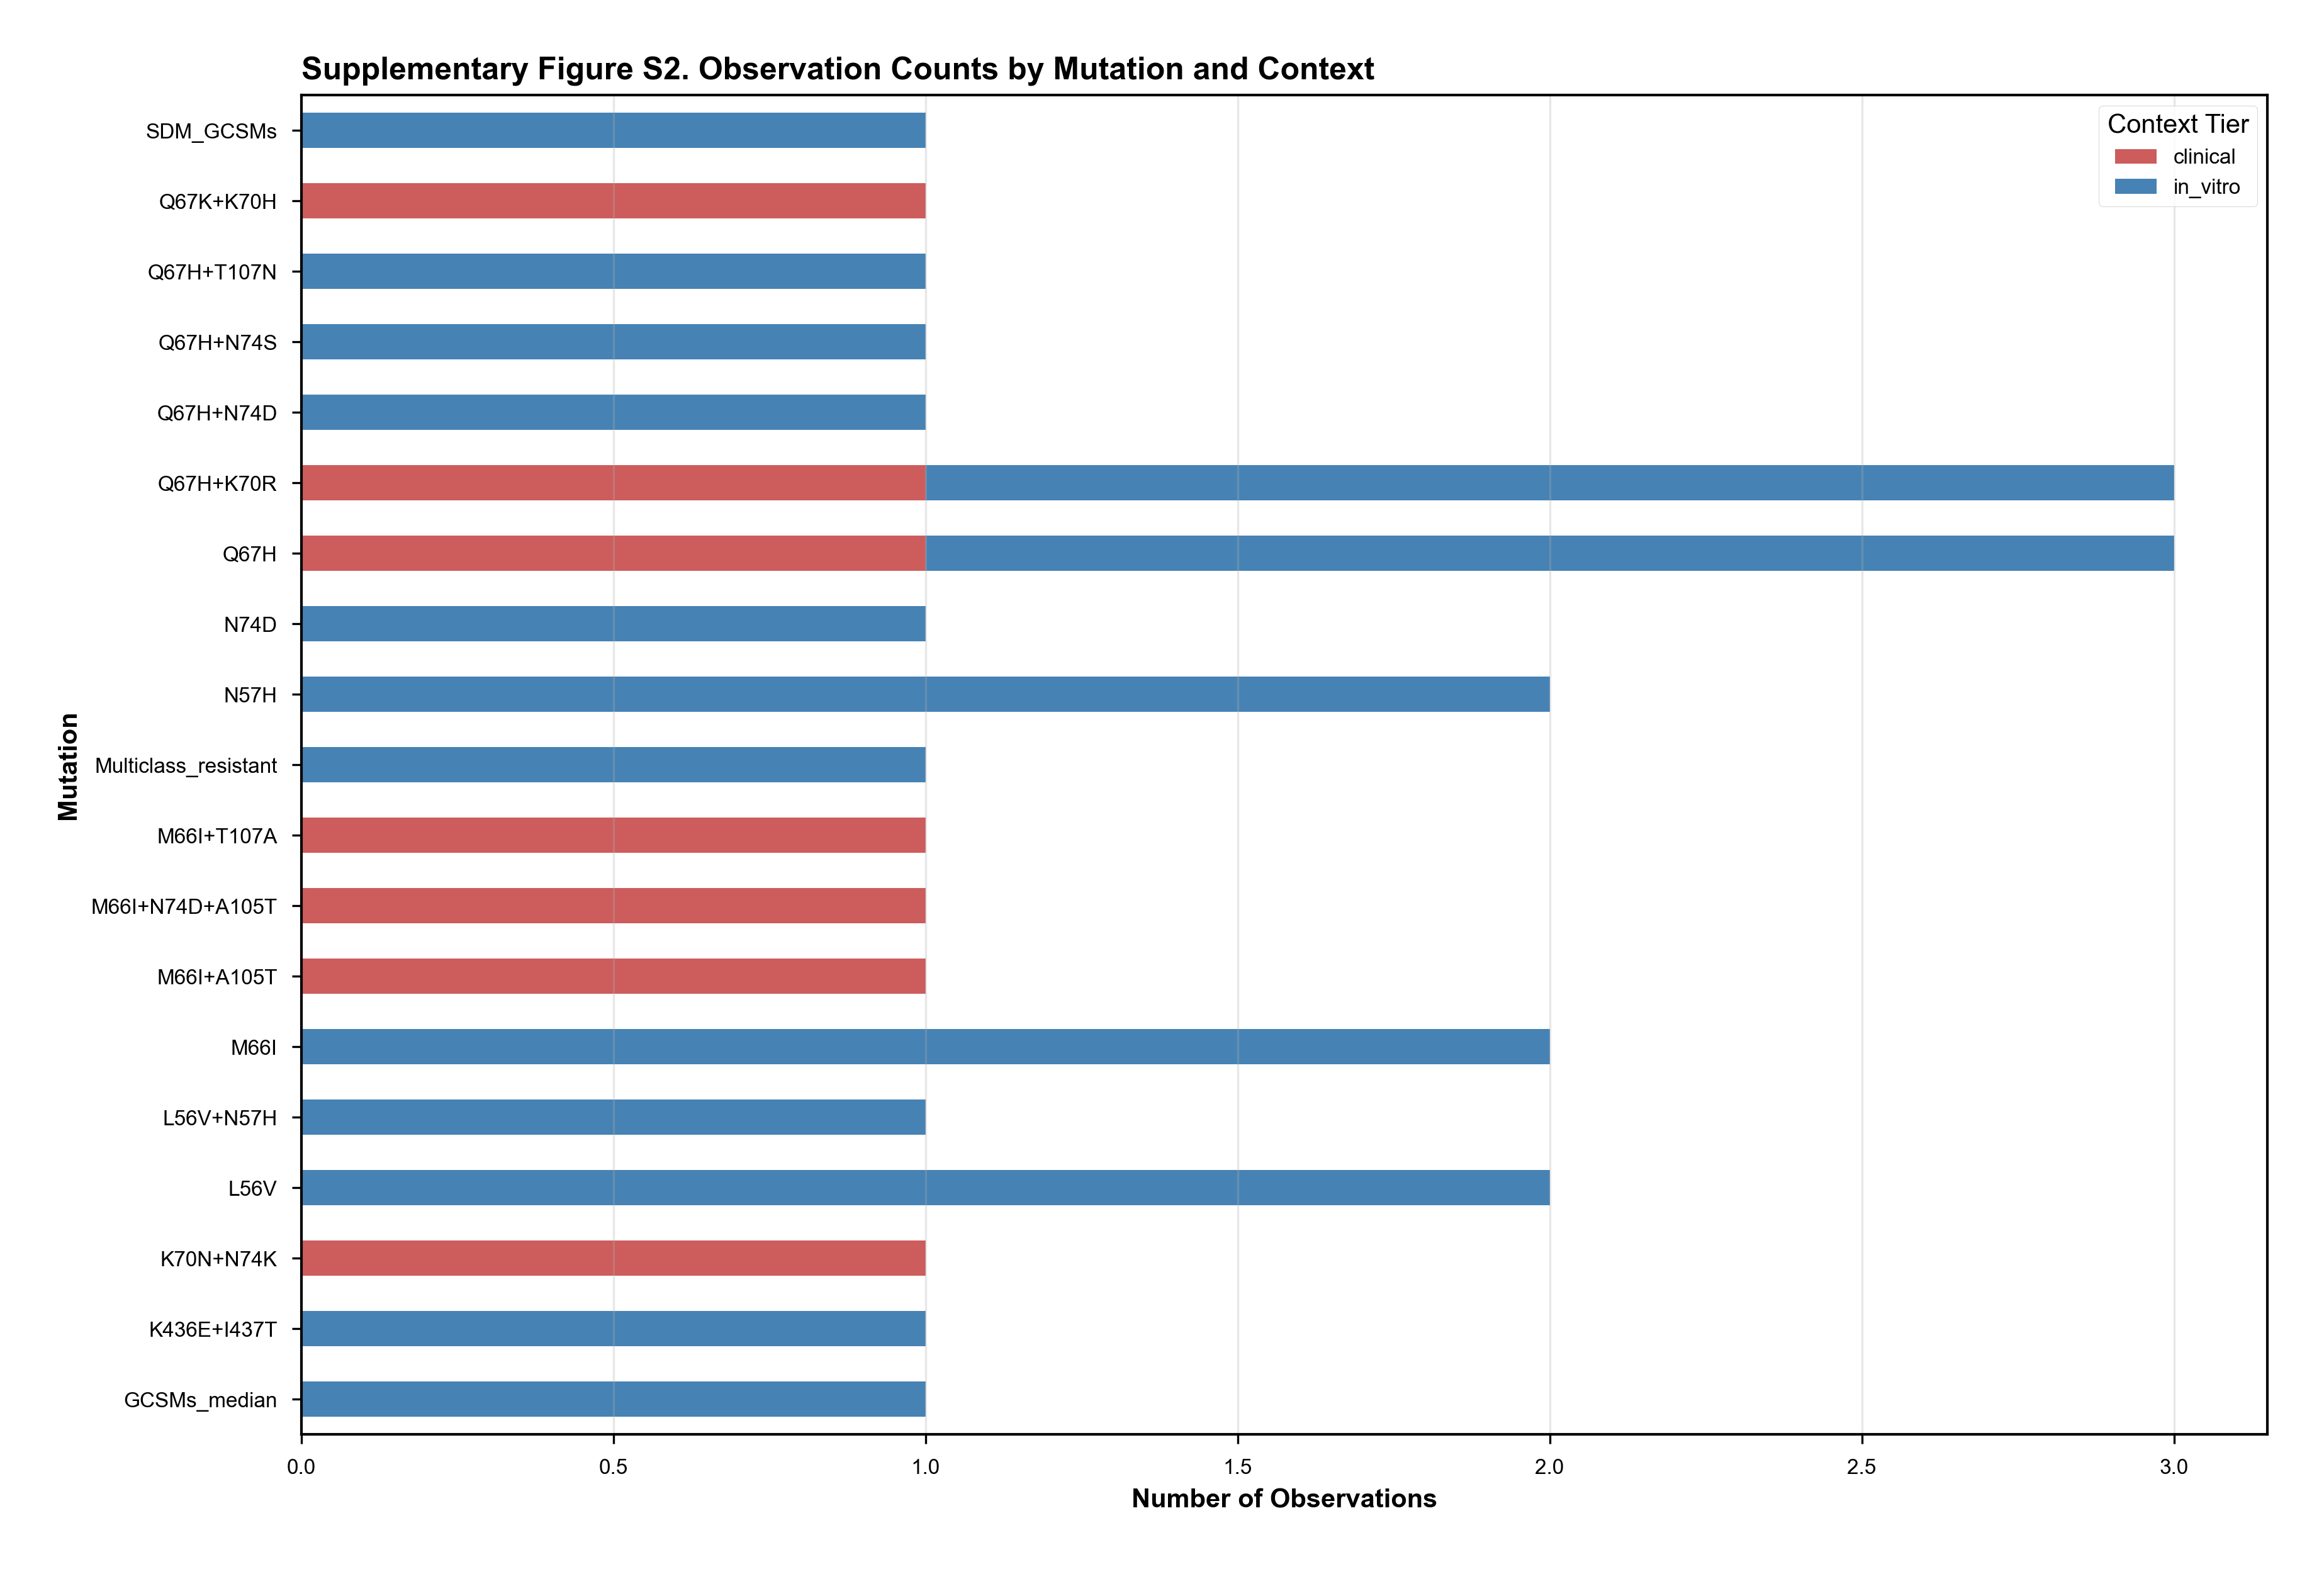
\includegraphics[width=0.85\textwidth]{supplementary/figures/figure_s2_observation_counts.pdf}
\caption{\textbf{Observation Counts by Mutation and Context.}
Stacked bar chart showing the number of observations for each mutation stratified by context tier (clinical, in vitro, natural polymorphism). Mutation labels are shown on the y-axis.}
\label{fig:s2}
\end{figure}

\newpage

% ============================================================
% FIGURE S3
% ============================================================
\begin{figure}[!ht]
\centering
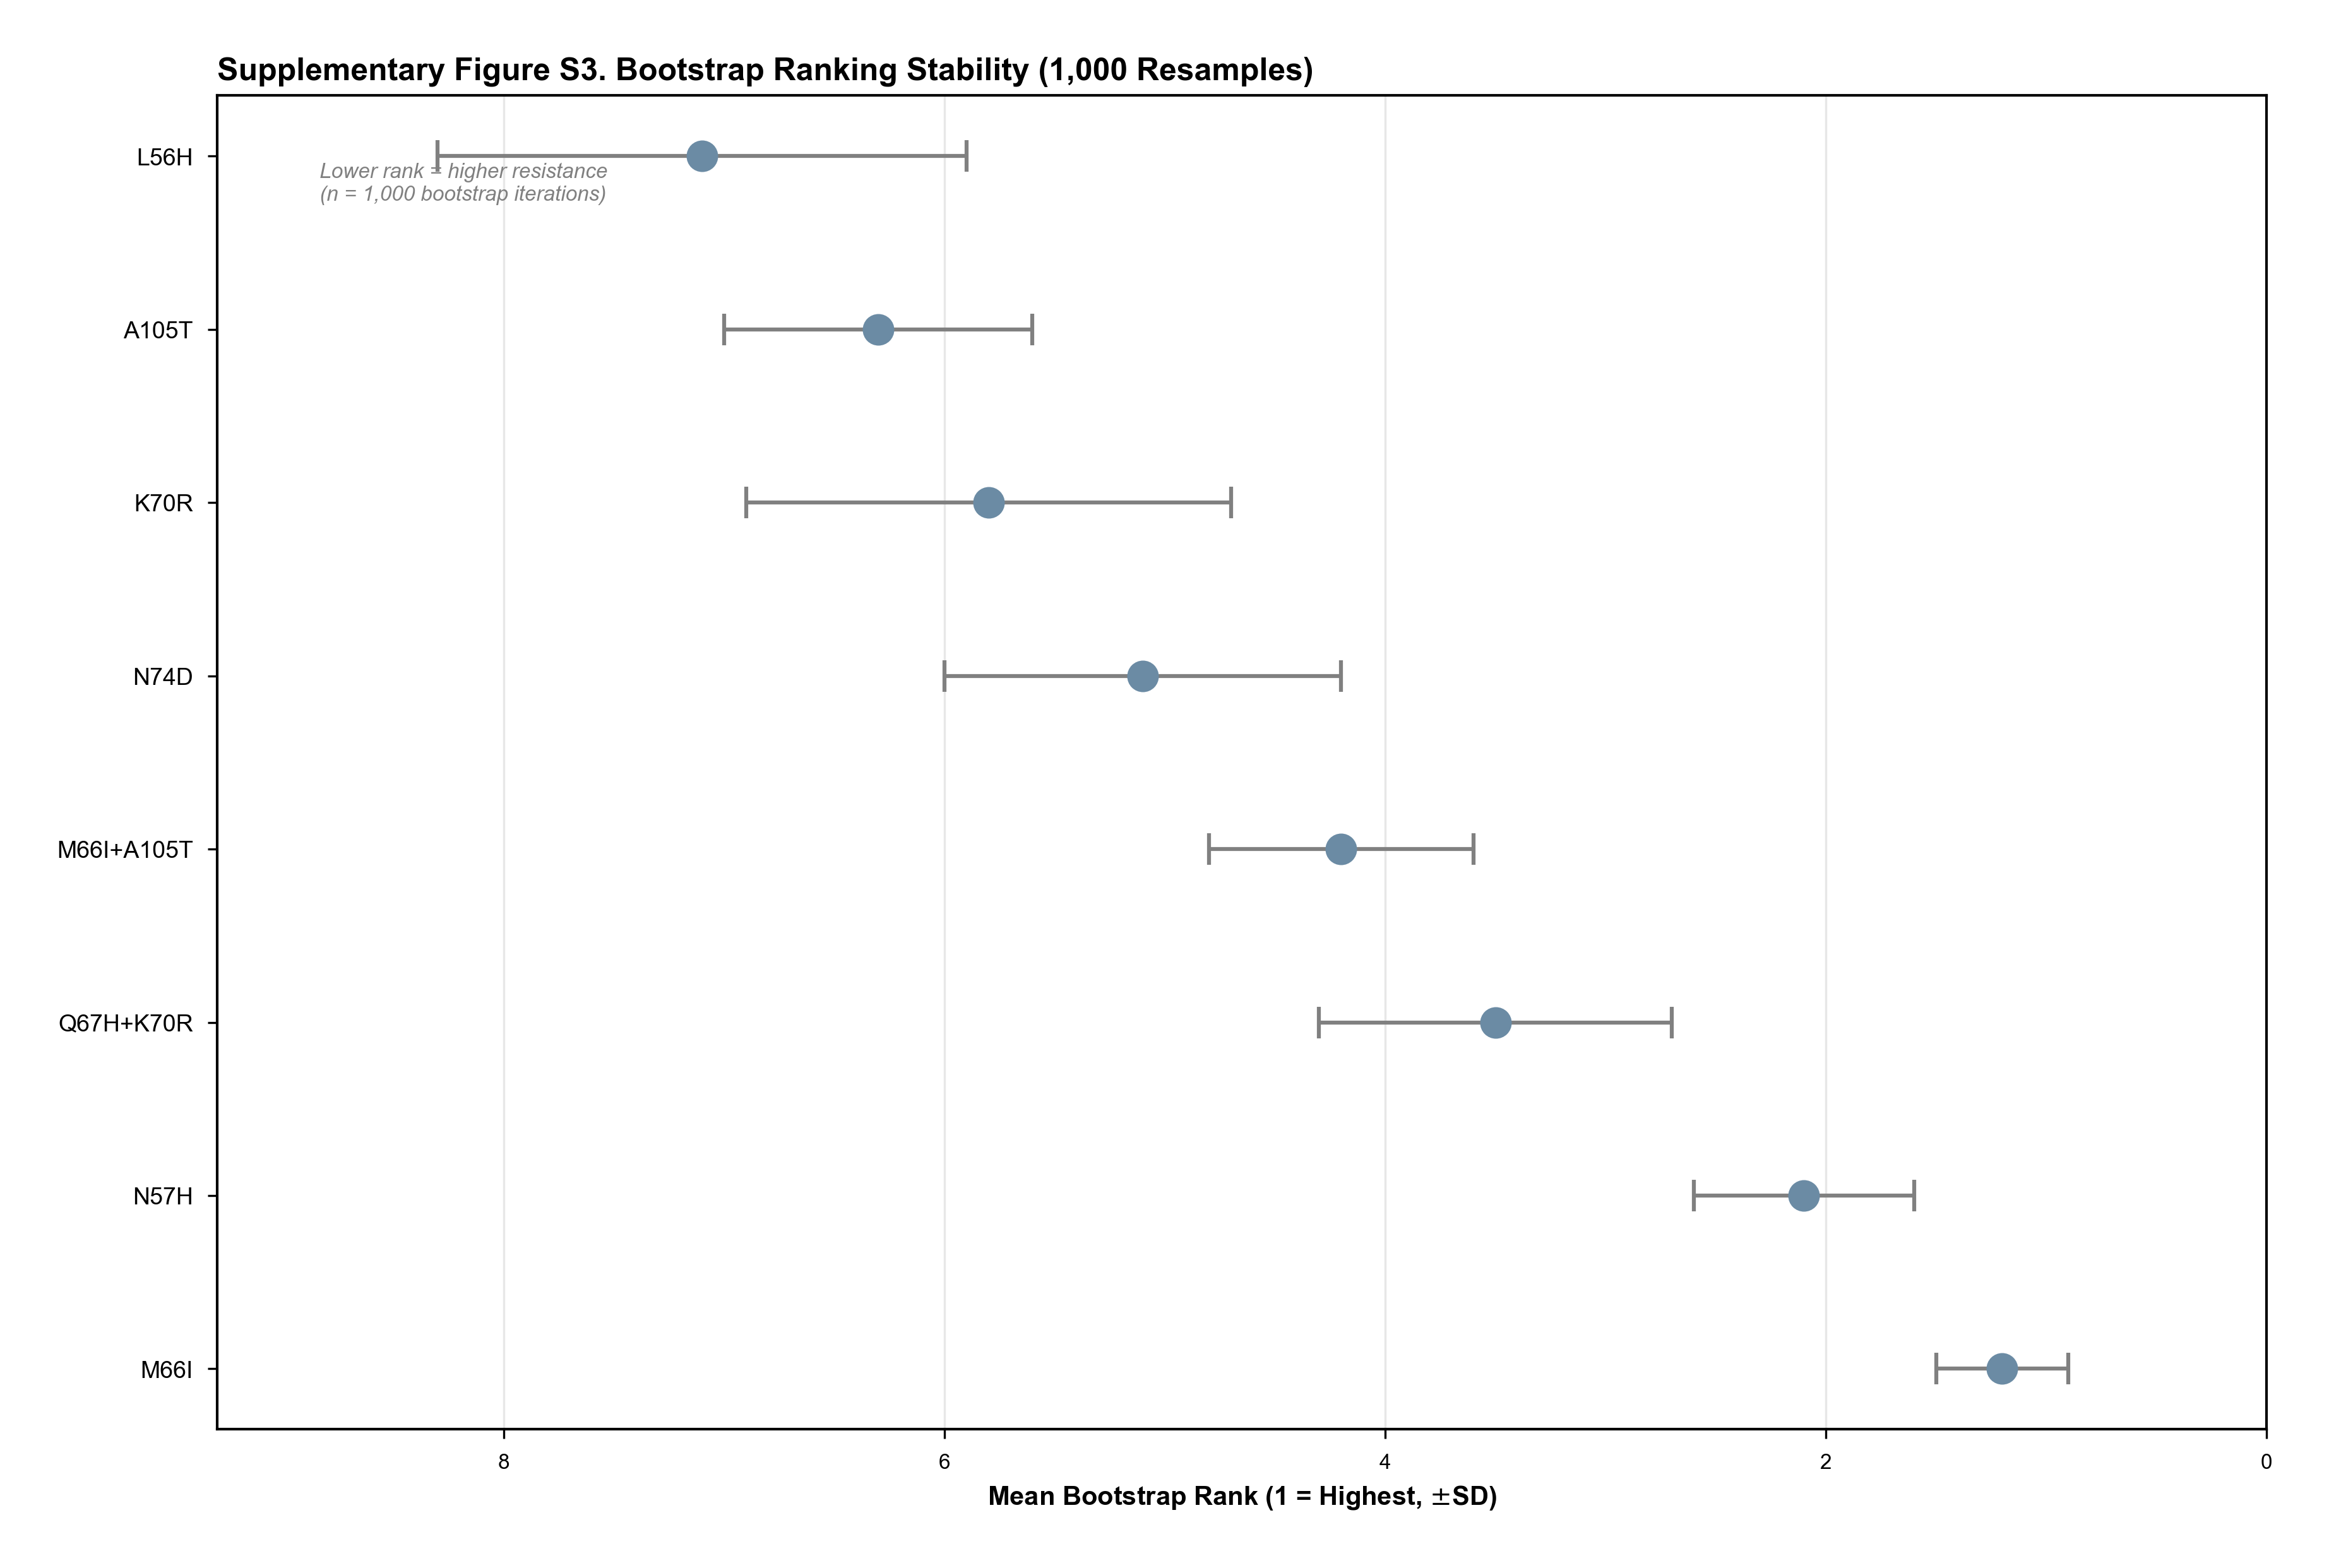
\includegraphics[width=0.9\textwidth]{supplementary/figures/figure_s3_bootstrap.pdf}
\caption{\textbf{Bootstrap Ranking Stability.}
Cleveland dot plot showing mean bootstrap rank ($\pm$ standard deviation) for 8 key mutations across 1,000 resamplings. Lower rank indicates higher resistance. N57H and M66I show the most stable top rankings (mean ranks 1.0 and 1.9, respectively).}
\label{fig:s3}
\end{figure}

\newpage

% ============================================================
% FIGURE S4
% ============================================================
\begin{figure}[!ht]
\centering
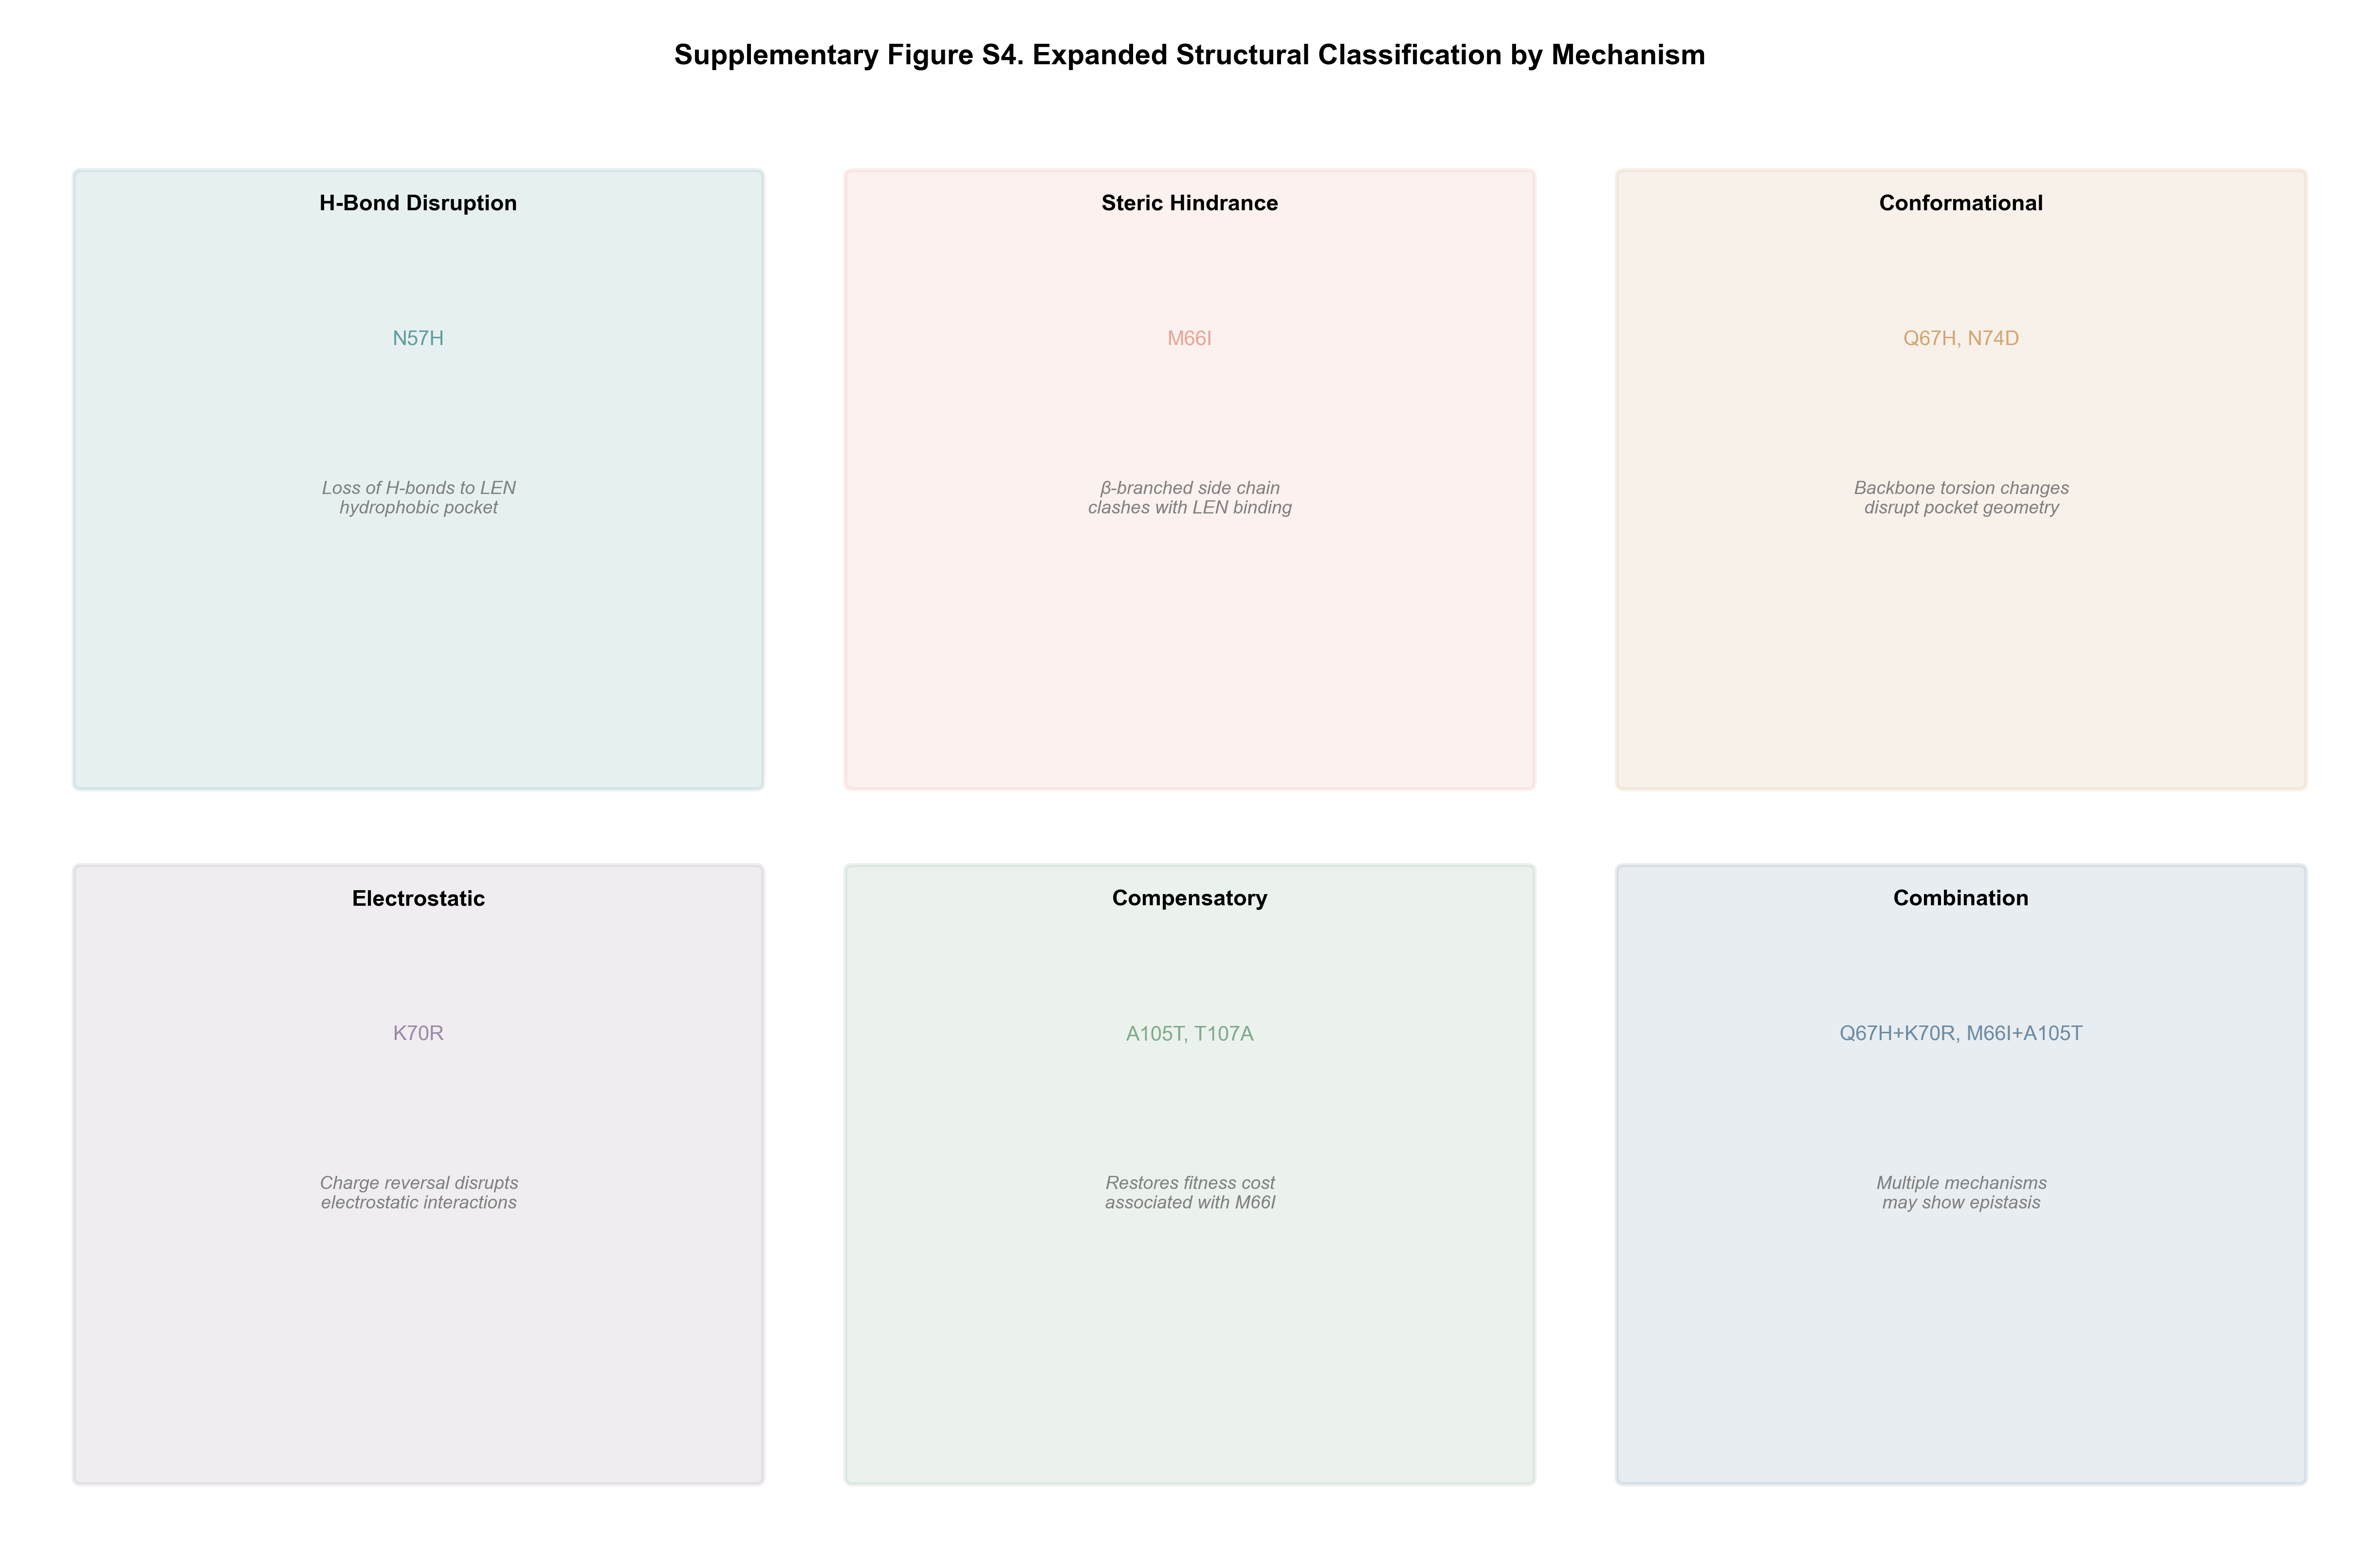
\includegraphics[width=0.95\textwidth]{supplementary/figures/figure_s4_structural.pdf}
\caption{\textbf{Expanded Structural Classification by Mechanism.}
Six-panel visualization showing mutation groupings by mechanistic class: H-bond disruption (N57H), steric hindrance (M66I), conformational (Q67H, N74D), electrostatic (K70R), compensatory (A105T, T107A), and combination (Q67H+K70R, M66I+A105T). Each panel includes mechanism description.}
\label{fig:s4}
\end{figure}

\newpage

% ============================================================
% FIGURE S5
% ============================================================
\begin{figure}[!ht]
\centering
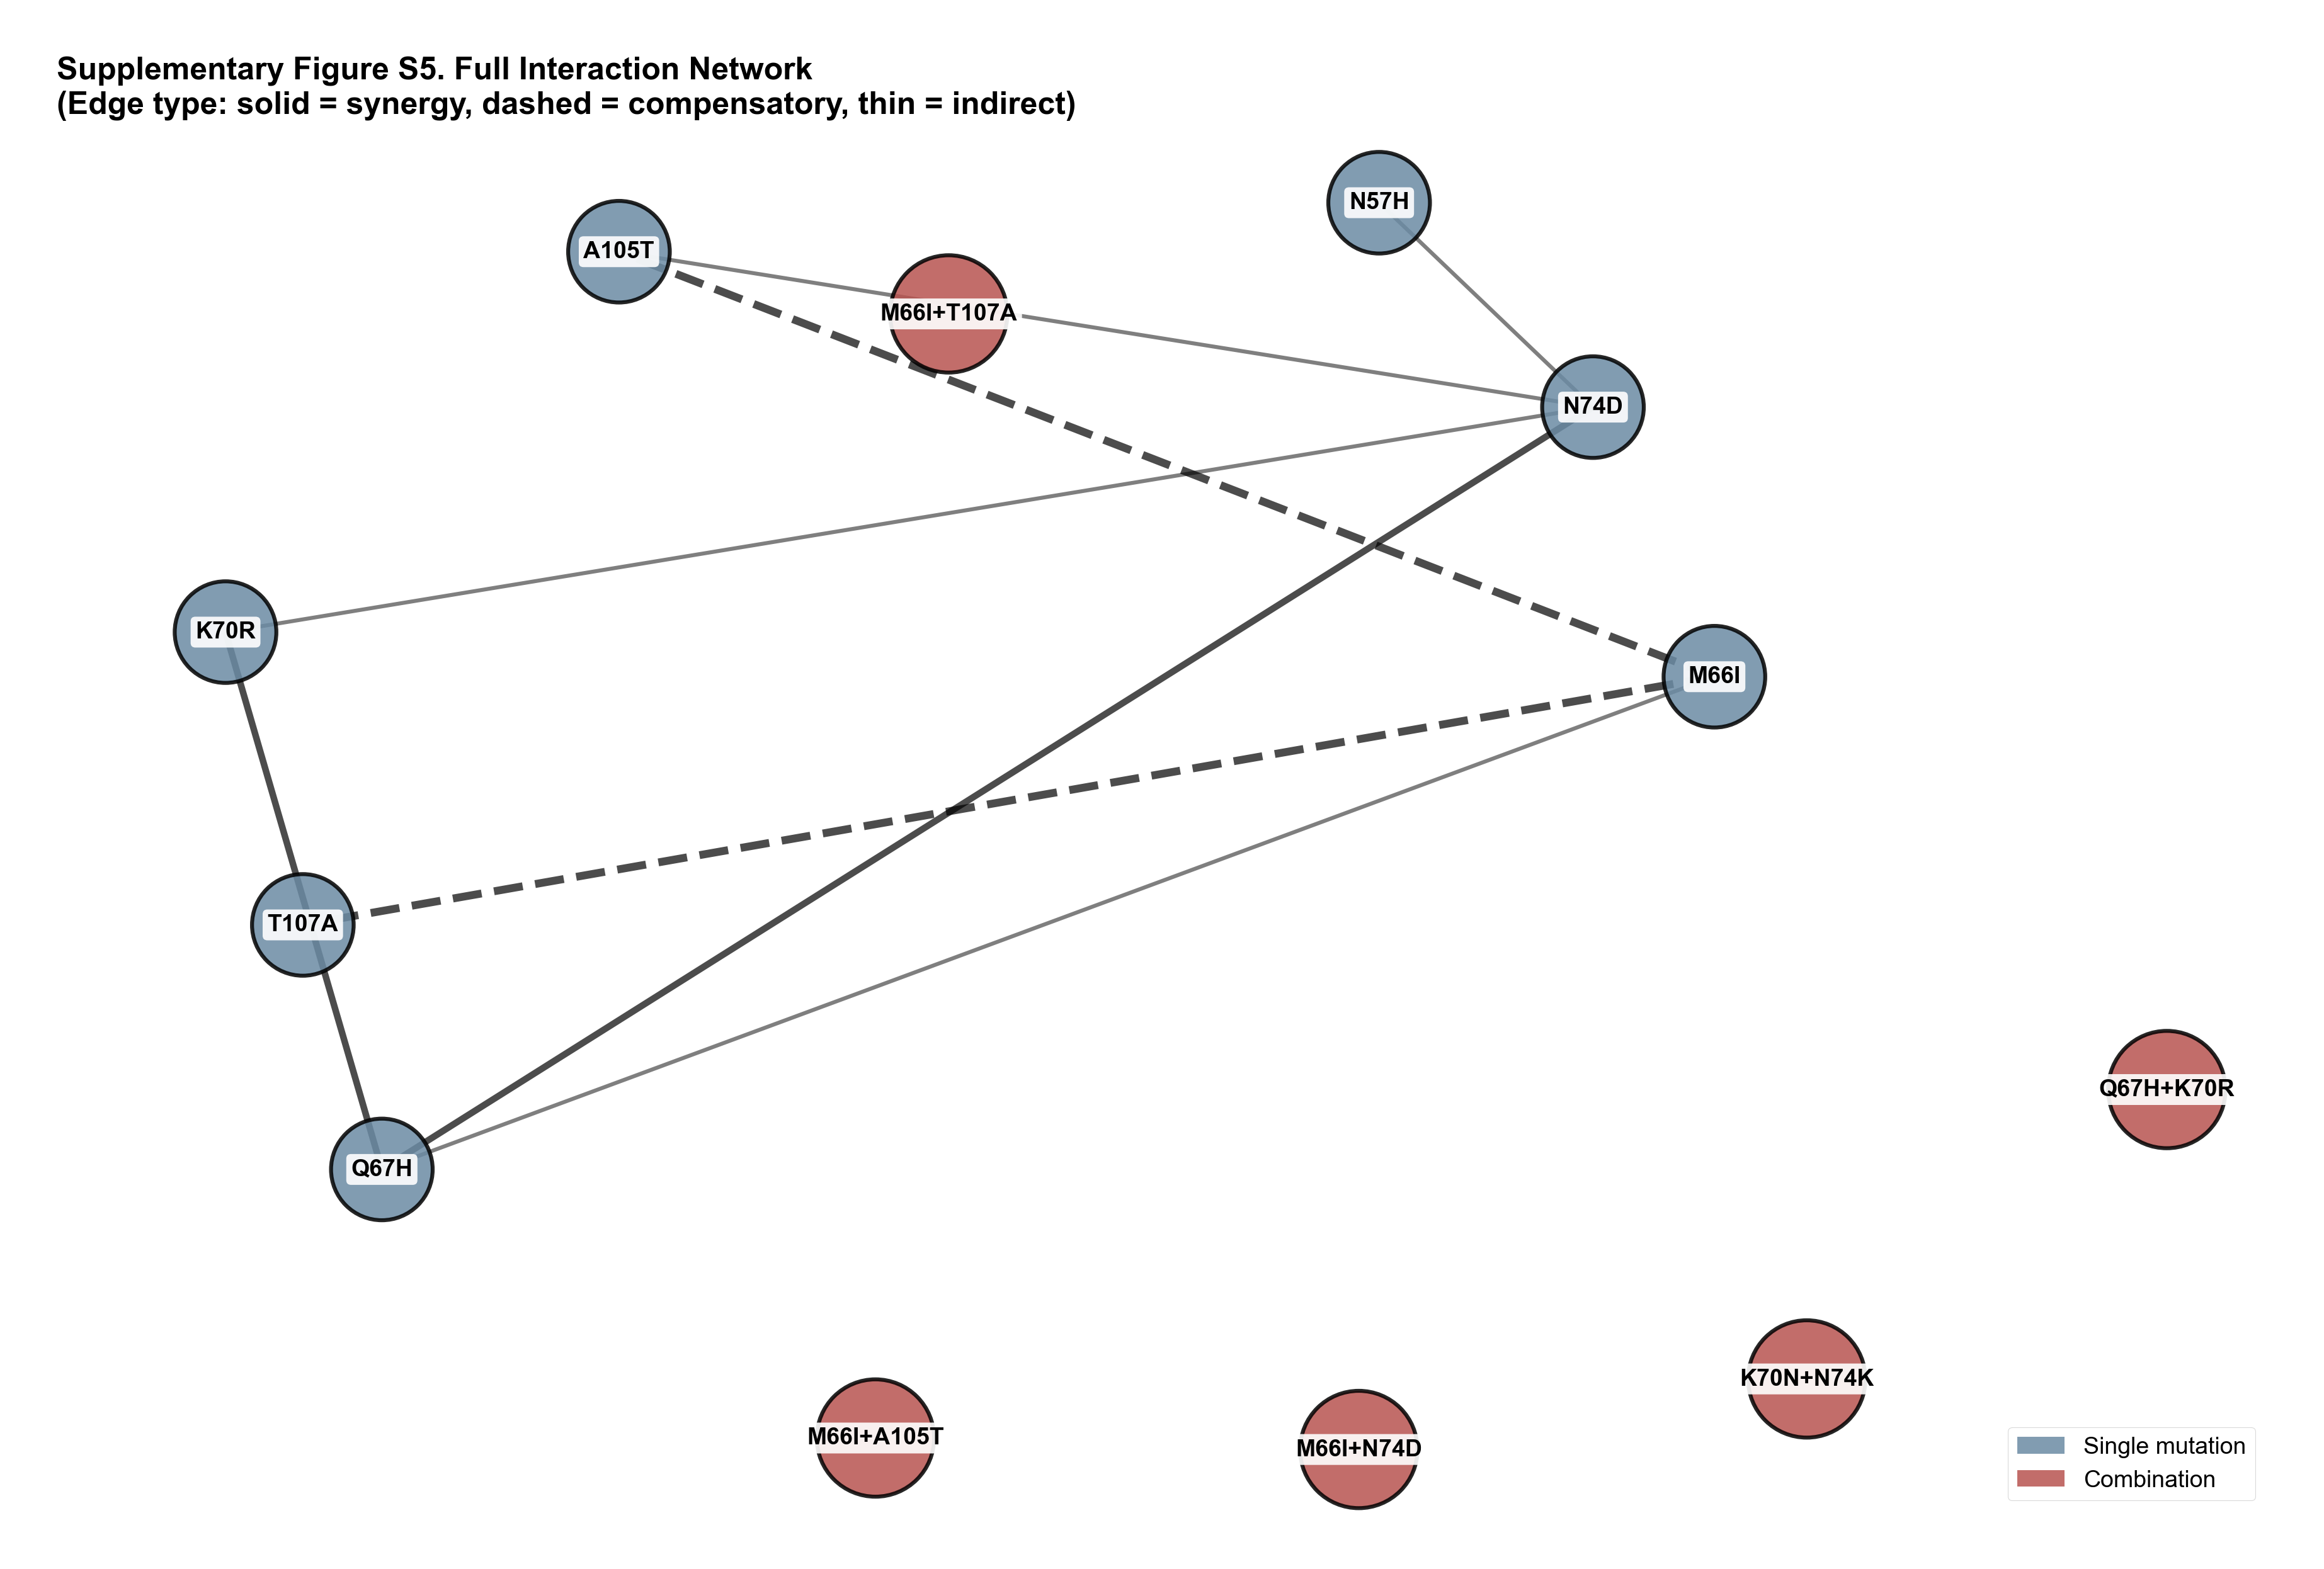
\includegraphics[width=0.85\textwidth]{supplementary/figures/figure_s5_network.pdf}
\caption{\textbf{Full Interaction Network.}
Network graph visualization of epistatic interactions among LEN resistance mutations. Single mutations are shown as smaller blue-gray nodes; combination mutations as larger red nodes. Edge types indicate: solid = synergy, dashed = compensatory, thin = indirect interaction.}
\label{fig:s5}
\end{figure}

\newpage

% ============================================================
% FIGURE S6
% ============================================================
\begin{figure}[!ht]
\centering
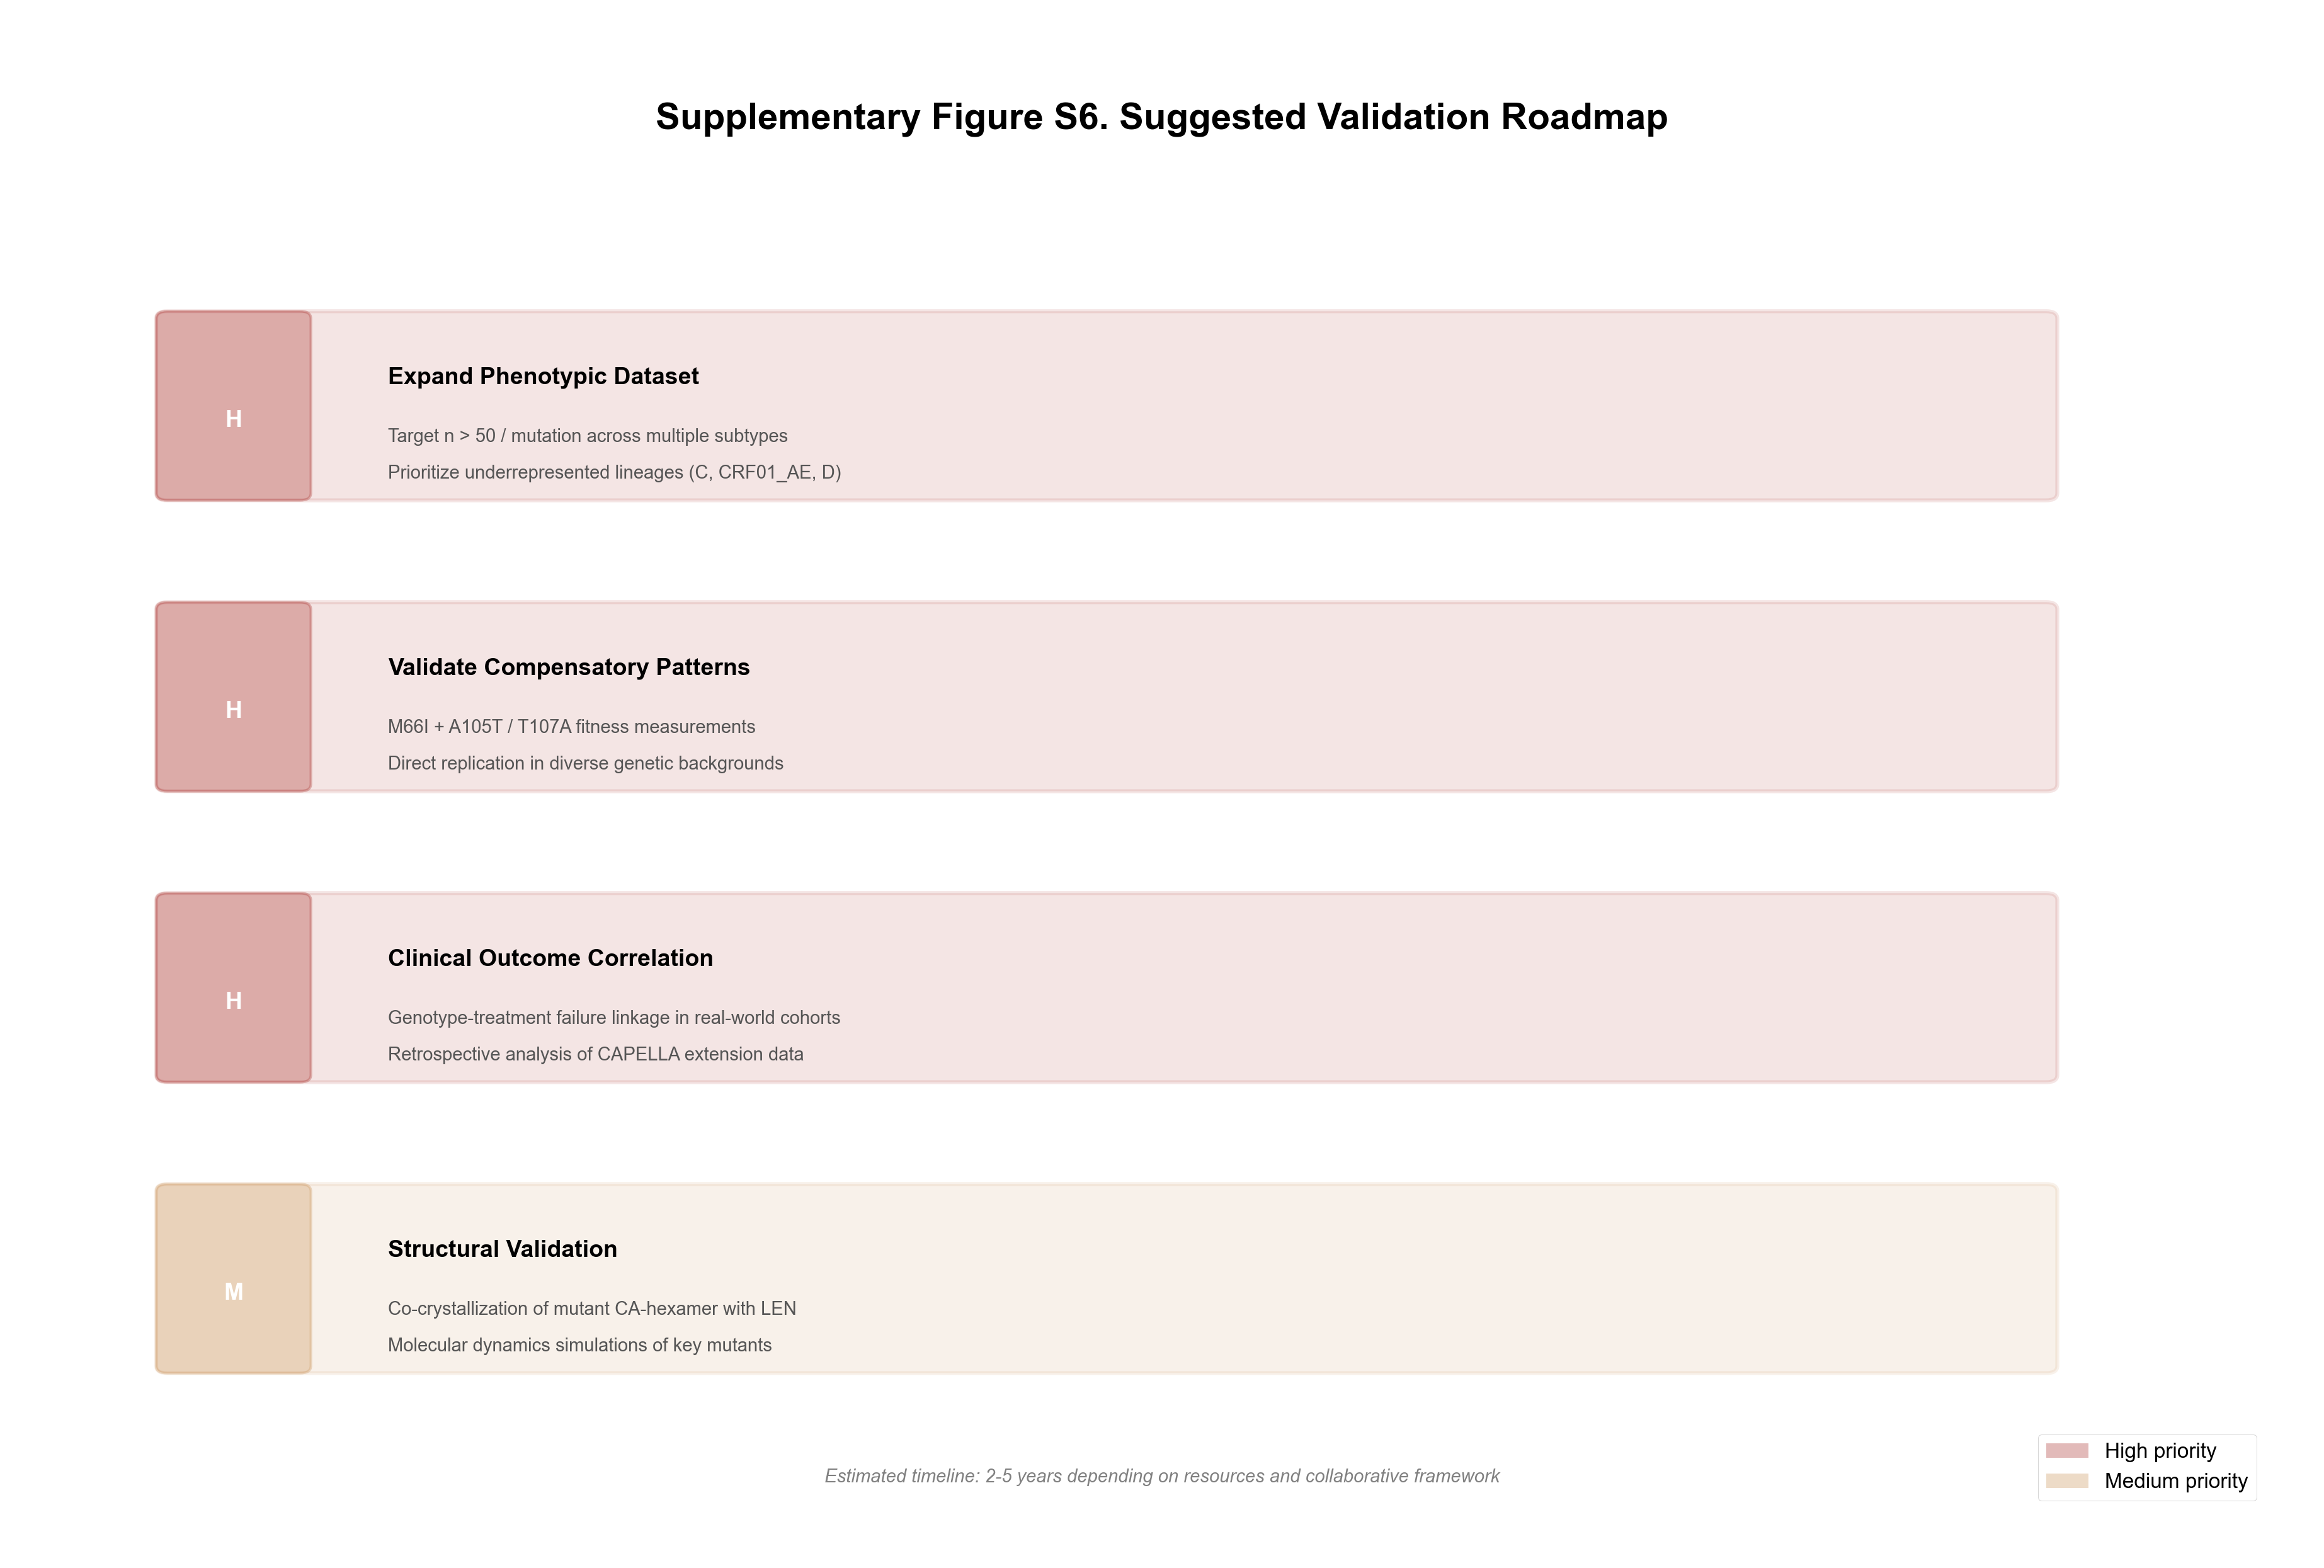
\includegraphics[width=0.8\textwidth]{supplementary/figures/figure_s6_roadmap.pdf}
\caption{\textbf{Validation Roadmap.}
Prioritized next steps for expanding the evidence base, including estimated feasibility and required sample sizes for quantifying subtype contribution beyond mutation-level effects.}
\label{fig:s6}
\end{figure}

\newpage

% ============================================================
% FIGURE S7
% ============================================================
\begin{figure}[!ht]
\centering
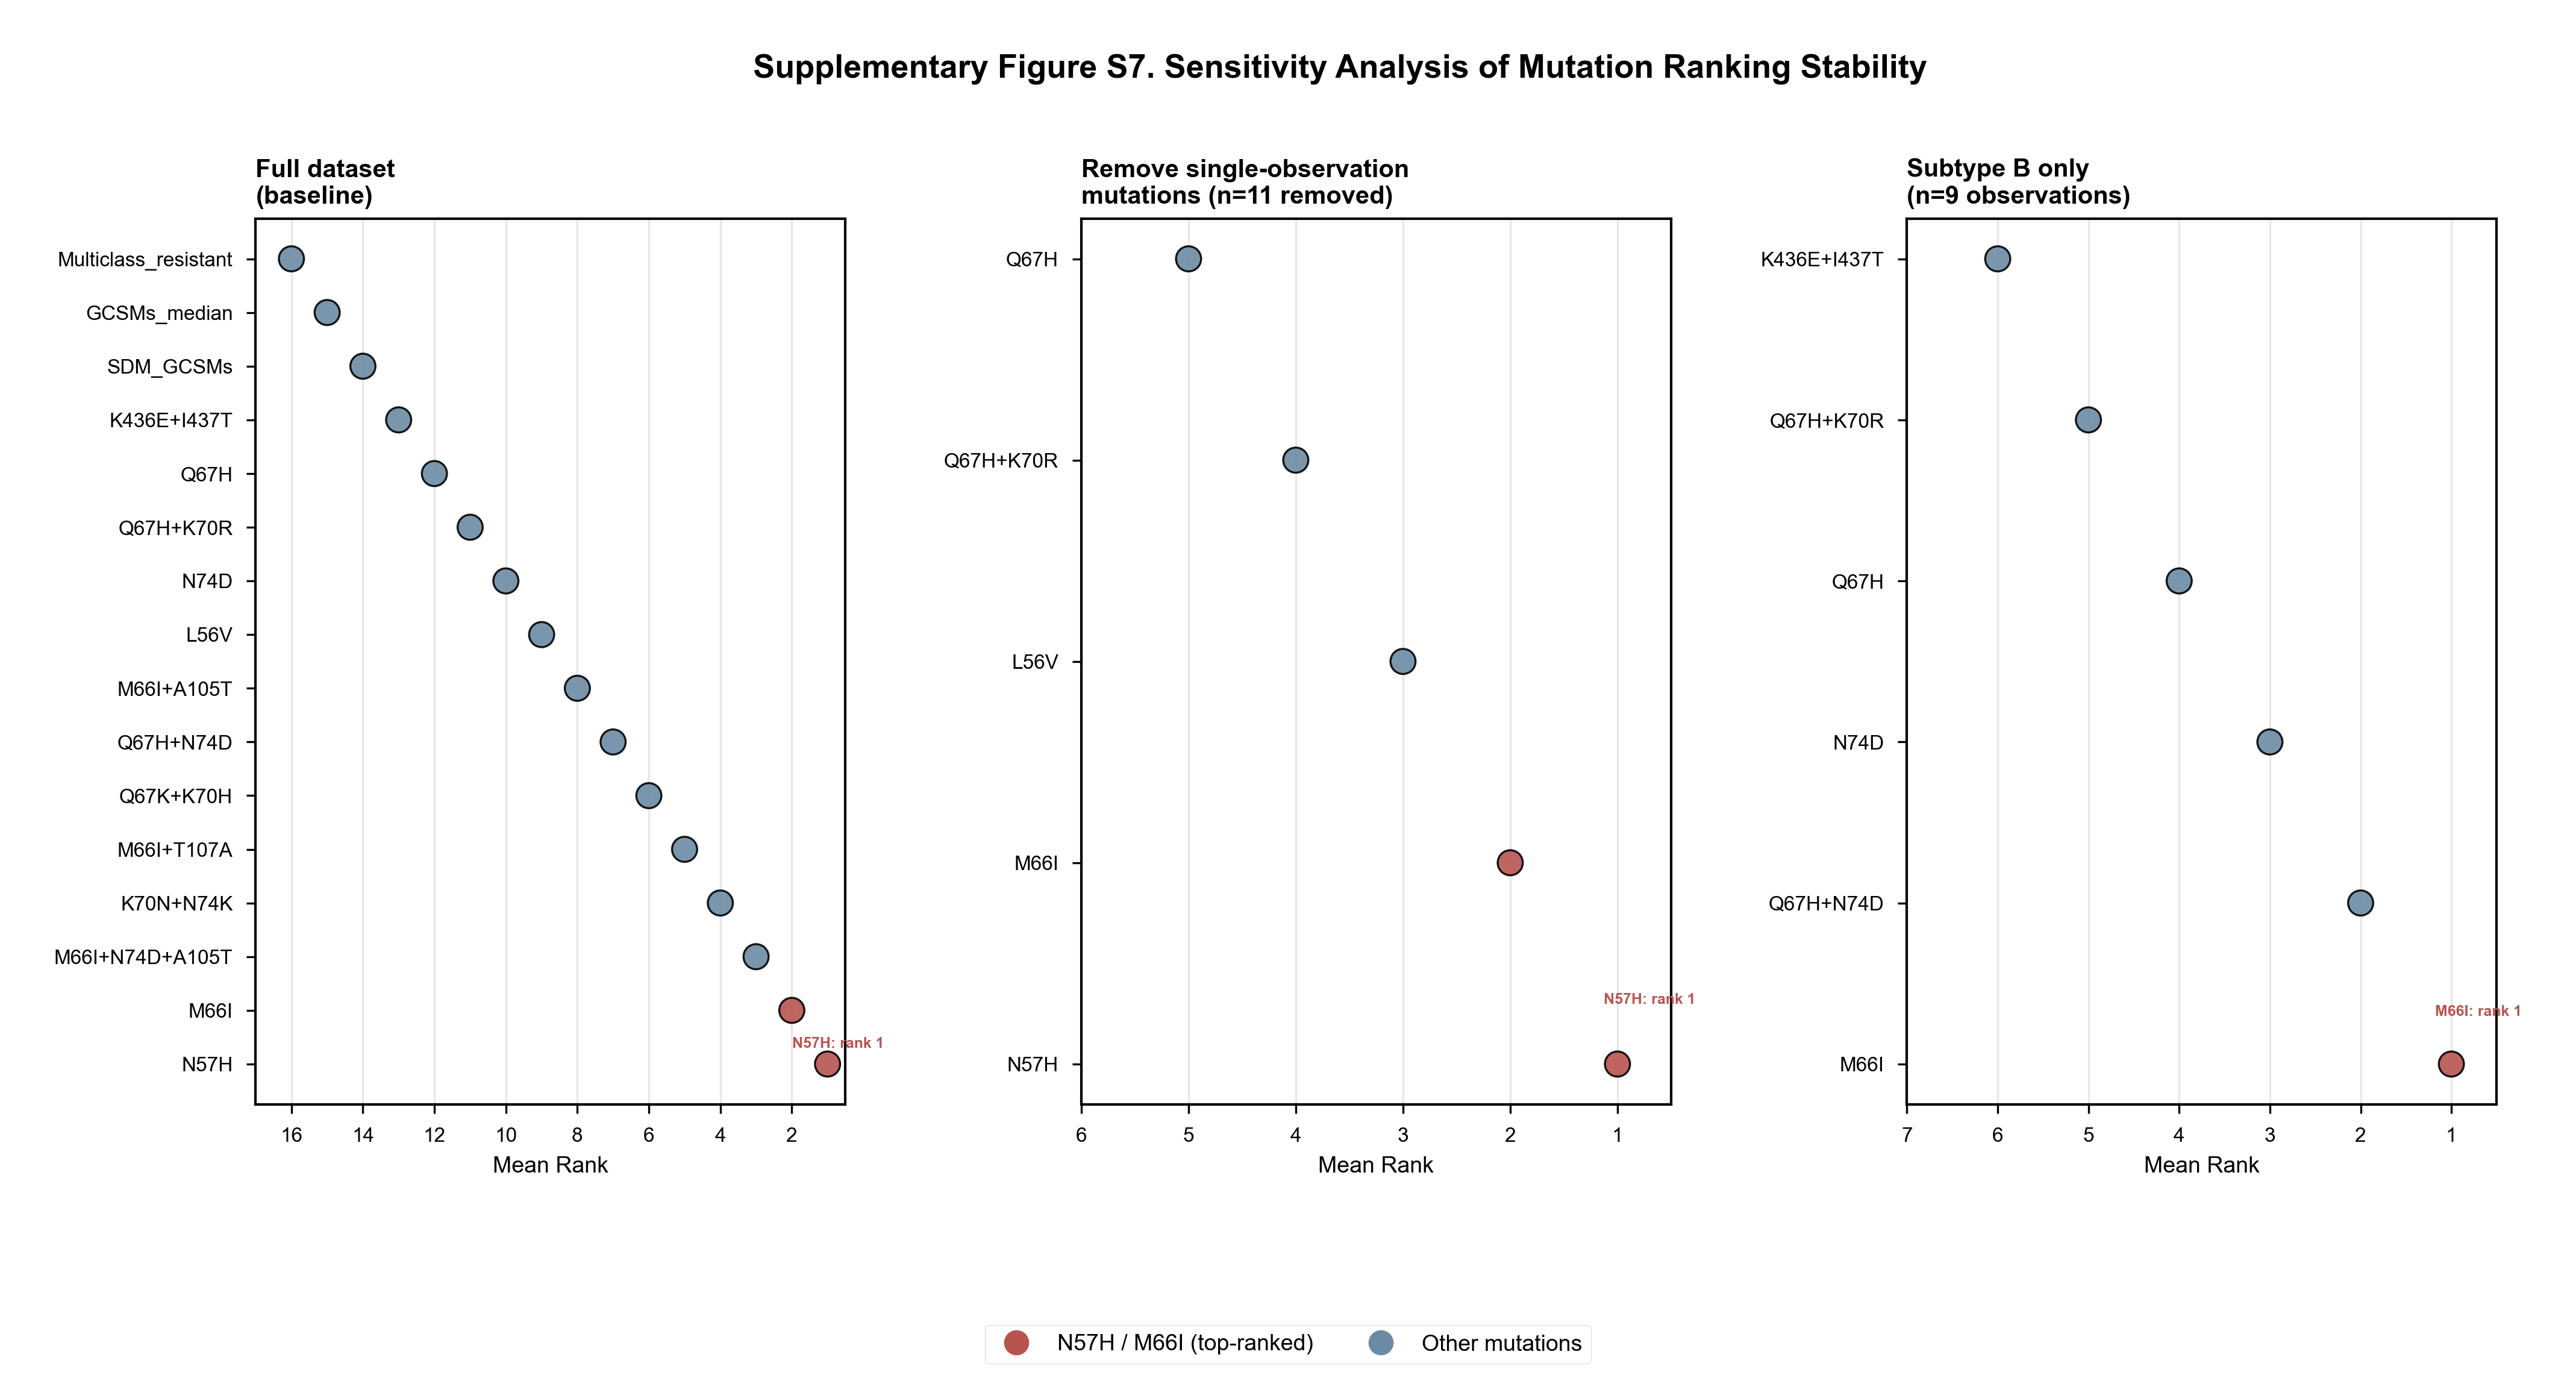
\includegraphics[width=0.95\textwidth]{supplementary/figures/figure_s7_sensitivity.pdf}
\caption{\textbf{Sensitivity Analysis of Mutation Ranking Stability.}
Cleveland dot plots showing mean rank ($\pm$ SD) for mutations across three data perturbations: (left) full dataset (baseline), (center) removing single-observation mutations, (right) subtype B only. N57H and M66I remain the top-ranked mutations under all perturbations, supporting ranking robustness.}
\label{fig:s7}
\end{figure}

\newpage

% ============================================================
% TABLE S2
% ============================================================
\begin{table}[!ht]
\centering
\caption{\textbf{Genetic Barrier Scores for LEN Resistance-Associated Mutations.}}
\label{tab:s2}
\vspace{0.3cm}
{\small
\resizebox{\textwidth}{!}{%
\begin{tabular}{lcccc}
\toprule
\textbf{Mutation} & \textbf{Codon Changes} & \textbf{Score} & \textbf{Class} & \textbf{Fitness} \\
\midrule
N57H       & 1 & 2.5 & Low    & Low \\
M66I       & 1 & 1.5 & Low    & High \\
Q67H       & 1 & 2.5 & Low    & Low \\
K70R       & 1--2 & 1.0--3.0 & Low    & Low \\
K70N       & 1 & 2.5 & Low    & Moderate \\
N74D       & 1 & 2.5 & Low    & Moderate \\
A105T      & 1--2 & 2.5--4.5 & Low--Moderate & Low \\
A105V      & 1--2 & 1.0--3.0 & Low    & Moderate \\
T107A      & 1 & 2.5 & Low    & Low \\
\midrule
Q67H+K70R  & 2 & 3.0 & Low    & High \\
Q67H+N74D  & 2 & 3.0 & Low    & High \\
M66I+A105T & 2 & 3.0 & Low    & High \\
M66I+T107A & 2 & 3.0 & Low    & High \\
A105T+T107A & 2 & 3.0 & Low    & High \\
\bottomrule
\end{tabular}%
}

\vspace{0.2cm}
\par\noindent\footnotesize\textit{Note:} Barrier score $= n_{\text{transversions}} \times 2 \allowbreak + n_{\text{transitions}} \allowbreak \pm \sum \text{property\_penalties}$. A105T and K70R have subtype-specific codon variations that increase barrier score in some genetic backgrounds (e.g., A105T: 4.5 in subtype C; K70R: 3.0 in subtype C via AAG$\rightarrow$AGA). Barrier classification: High ($\geq$7), Moderate (4--6), Low ($<$4).
}

\end{table}

\newpage

% ============================================================
% TABLE S3
% ============================================================
\begin{table}[!ht]
\centering
\caption{\textbf{Study Characteristics of Included Publications ($n=7$).}}
\label{tab:s3}
\vspace{0.3cm}
{\setlength{\tabcolsep}{4pt}%
\footnotesize
\resizebox{\textwidth}{!}{%
\begin{tabular}{llrcllc}
\toprule
\textbf{Study ID} & \textbf{First Author} & \textbf{Year} & \textbf{Mutations Reported} & \textbf{N} & \textbf{Context} & \textbf{Assay} \\
\midrule
PMC12077089 & Andreatta        & 2024 & L56V, N57H                                    & 2 & In vitro selection  & MT-2 cells   \\
PMC9600929  & Yant             & 2022 & M66I, Q67H, N74D, Q67H+N74D, Q67H+K70R       & 5 & In vitro SDM       & MT-4 cells   \\
JID2025     & CAPELLA group    & 2025 & M66I+N74D+A105T, K70N+N74K, Q67H+K70R        & 3 & Clinical isolate   & PBMC         \\
JAC2025     & Uganda study     & 2025 & Q67H+K70R                                     & 1 & Natural polymorphism & Phenotypic assay \\
NATAP2022   & Margot           & 2022 & Q67H, N74D, K70R                              & 3 & Clinical isolate   & MT-4 cells   \\
PMC8092519  & Link             & 2021 & M66I                                          & 1 & In vitro SDM       & MT-4 cells   \\
EMJ2025     & EMJ clinical     & 2025 & Q67H                                          & 1 & Clinical           & Unknown      \\
\bottomrule
\end{tabular}%
}
}
\end{table}

\newpage

% ============================================================
% TABLE S4
% ============================================================
\begin{table}[!ht]
\centering
\caption{\textbf{Per-Mutation Summary Statistics of Phenotypic Observations.}}
\label{tab:s4}
\vspace{0.3cm}
{\small
\resizebox{\textwidth}{!}{%
\begin{tabular}{lrrlrrrrr}
\toprule
\textbf{Mutation} & \textbf{N obs} & \textbf{N studies} & \textbf{Contexts} & \textbf{Mean log$_{10}$FC} & \textbf{SD} & \textbf{Min} & \textbf{Max} & \textbf{Mean Quality} \\
\midrule
N57H            & 2 & 1 & in\_vitro         & 3.689 & 0.000 & 3.689 & 3.689 & 3.0 \\
M66I            & 2 & 2 & in\_vitro         & 3.505 & 0.000 & 3.505 & 3.505 & 3.0 \\
K70N+N74K       & 1 & 1 & clinical          & 2.461 & ---   & 2.461 & 2.461 & 5.0 \\
M66I+N74D+A105T & 1 & 1 & clinical          & 3.126 & ---   & 3.126 & 3.126 & 3.0 \\
Q67H            & 3 & 3 & clinical, in\_vitro & 0.716 & 0.055 & 0.672 & 0.778 & 3.0 \\
L56V            & 2 & 1 & in\_vitro         & 1.857 & 0.000 & 1.857 & 1.857 & 3.0 \\
M66I+T107A      & 1 & 1 & clinical          & 2.369 & ---   & 2.369 & 2.369 & 5.0 \\
M66I+A105T      & 1 & 1 & clinical          & 2.045 & ---   & 2.045 & 2.045 & 5.0 \\
Q67H+N74D       & 1 & 1 & in\_vitro         & 2.176 & ---   & 2.176 & 2.176 & 3.0 \\
N74D            & 1 & 1 & in\_vitro         & 1.301 & ---   & 1.301 & 1.301 & 3.0 \\
Q67H+K70R       & 3 & 3 & clinical, in\_vitro & 0.893 & 0.995 & --0.229 & 1.666 & 4.3 \\
Q67K+K70H       & 1 & 1 & clinical          & 2.223 & ---   & 2.223 & 2.223 & 5.0 \\
K436E+I437T     & 1 & 1 & in\_vitro         & 0.204 & ---   & 0.204 & 0.204 & 4.0 \\
\bottomrule
\end{tabular}%
}
}

\end{table}

\newpage

% ============================================================
% TABLE S5
% ============================================================
{\tiny
\setlength{\tabcolsep}{3pt}%
\begin{longtable}{p{1.3cm}p{1.8cm}rrp{1.0cm}p{1.5cm}cp{3.2cm}}
\caption{\textbf{Complete harmonized phenotype dataset ($n=27$ observations).}} \\
\toprule
\textbf{Source} & \textbf{Mutation} & \textbf{FC} & \textbf{log$_{10}$FC} & \textbf{Context} & \textbf{Subtype} & \textbf{Quality} & \textbf{Notes} \\
\midrule
\endfirsthead
\multicolumn{8}{c}{\tablename\ \thetable\ --- continued from previous page} \\
\toprule
\textbf{Source} & \textbf{Mutation} & \textbf{FC} & \textbf{log$_{10}$FC} & \textbf{Context} & \textbf{Subtype} & \textbf{Quality} & \textbf{Notes} \\
\midrule
\endhead
\bottomrule
\multicolumn{8}{r}{Continued on next page} \\
\endfoot
\bottomrule
\endlastfoot

NATAP2022     & Q67H              & 6.0    & 0.778 & In\_vitro & B             & 3 & Low-level resistance \\
PMC8092519    & GCSMs\_median     & 0.8    & --0.097 & In\_vitro & Mixed         & 3 & Treatment-naive isolates \\
PMC8092519    & SDM\_GCSMs        & 1.0    & 0.000 & In\_vitro & Mixed         & 3 & Site-directed mutagenesis \\
PMC8092519    & Multiclass\_resistant & 0.65 & --0.187 & In\_vitro & Mixed       & 3 & No cross-resistance \\
PMC12077089   & L56V              & 72.0   & 1.857 & In\_vitro & Mixed         & 3 & Steric clash with di-fluoro-benzyl \\
PMC12077089   & N57H              & 4890.0 & 3.689 & In\_vitro & Mixed         & 3 & H-bond loss \\
EMJ2025       & Q67H              & 4.7    & 0.672 & Clinical & Mixed         & 3 & Participant-developed Q67H \\
Structural\_2025 & M66I           & 3200.0 & 3.505 & In\_vitro & B             & 3 & KFA-027 vs M66I, 20-fold improvement over LEN \\
PMID40231850  & M66I              & 3200.0 & 3.505 & In\_vitro & B             & 3 & Highest resistance, steric hindrance \\
PMC9600929    & Q67H              & 5.0    & 0.699 & In\_vitro & B             & 3 & Kd fold change, dissociation rate affected \\
PMC9600929    & N74D              & 20.0   & 1.301 & In\_vitro & B             & 3 & Kd fold change, both kon and koff affected \\
PMC9600929    & Q67H+N74D         & 150.0  & 2.176 & In\_vitro & B             & 3 & Double mutant synergy \\
PMC9600929    & Q67H+K70R         & 0.59   & --0.229 & In\_vitro & B           & 3 & 1.7-fold improved potency with KFA-012 \\
PMC12077089   & L56V              & 72.0   & 1.857 & In\_vitro & CRF02\_AG     & 3 & Steric clash \\
PMC12077089   & N57H              & 4890.0 & 3.689 & In\_vitro & D             & 3 & H-bond loss with LEN \\
CAPELLA       & M66I+N74D+A105T   & 1337.0 & 3.126 & Clinical & Mixed         & 3 & Triple mutant with fitness restoration \\
JID2025       & M66I+A105T        & 111.0  & 2.045 & Clinical & Clinical isolate & 5 & CAPELLA Participant 7 \\
JID2025       & M66I+T107A        & 234.0  & 2.369 & Clinical & Clinical isolate & 5 & CAPELLA Participant 9 \\
JID2025       & Q67K+K70H         & 167.0  & 2.223 & Clinical & Clinical isolate & 5 & CAPELLA Participant 8 \\
JID2025       & K70N+N74K         & 289.0  & 2.461 & Clinical & Clinical isolate & 5 & CAPELLA Participant 11 \\
NATAP2022     & Q67H+T107N        & ---    & ---   & In\_vitro & B             & 4 & Combination variant \\
NATAP2022     & Q67H+N74S         & ---    & ---   & In\_vitro & B             & 4 & Combination variant \\
AAC\_2021     & K436E+I437T       & 1.6    & 0.204 & In\_vitro & B             & 4 & C-terminal domain double mutation \\
PMC12077089   & L56V+N57H         & ---    & ---   & In\_vitro & Primary T cells & 5 & Diminished replication \\
JAC2025       & Q67H+K70R         & 17.5   & 1.243 & In\_vitro & B             & 5 & Uganda A1/D subtype study \\
JID2025       & Q67H+K70R         & 46.3   & 1.666 & Clinical & Clinical isolate & 5 & CAPELLA Participant 5 \\
\end{longtable}
}

\newpage

% ============================================================
% TABLE S6
% ============================================================
\begin{table}[!ht]
\centering
\caption{\textbf{Multi-Mutant Phenotypic Observations.}}
\label{tab:s6}
\vspace{0.3cm}
{\setlength{\tabcolsep}{4pt}%
\footnotesize
\begin{tabular}{lrccll}
\toprule
\textbf{Mutation} & \textbf{FC} & \textbf{Context} & \textbf{Source} & \textbf{Subtype} & \textbf{Notes} \\
\midrule
Q67H+N74D   & 150.0  & In\_vitro & PMC9600929 & B             & Binding affinity reduction (SPR) \\
Q67H+K70R   & 0.59   & In\_vitro & PMC9600929 & B             & Improved potency with KFA-012 \\
Q67H+K70R   & 46.3   & Clinical & JID2025    & Clinical isolate & CAPELLA Participant 5 \\
Q67H+K70R   & 17.5   & In\_vitro & JAC2025    & B             & Uganda A1/D subtype study \\
M66I+A105T  & 111.0  & Clinical & JID2025    & Clinical isolate & CAPELLA Participant 7 \\
M66I+T107A  & 234.0  & Clinical & JID2025    & Clinical isolate & CAPELLA Participant 9 \\
Q67K+K70H   & 167.0  & Clinical & JID2025    & Clinical isolate & CAPELLA Participant 8 \\
K70N+N74K   & 289.0  & Clinical & JID2025    & Clinical isolate & CAPELLA Participant 11 \\
M66I+N74D+A105T & 1337.0 & Clinical & CAPELLA & Mixed & Triple mutant, fitness restoration \\
K436E+I437T & 1.6    & In\_vitro & AAC\_2021  & B             & C-terminal domain, non-LEN pocket \\
\bottomrule
\end{tabular}
}
\end{table}

\end{document}
